{
\begin{figure*}[th]
\begin{minipage}{0.50\columnwidth}
\begin{center}
\centerline{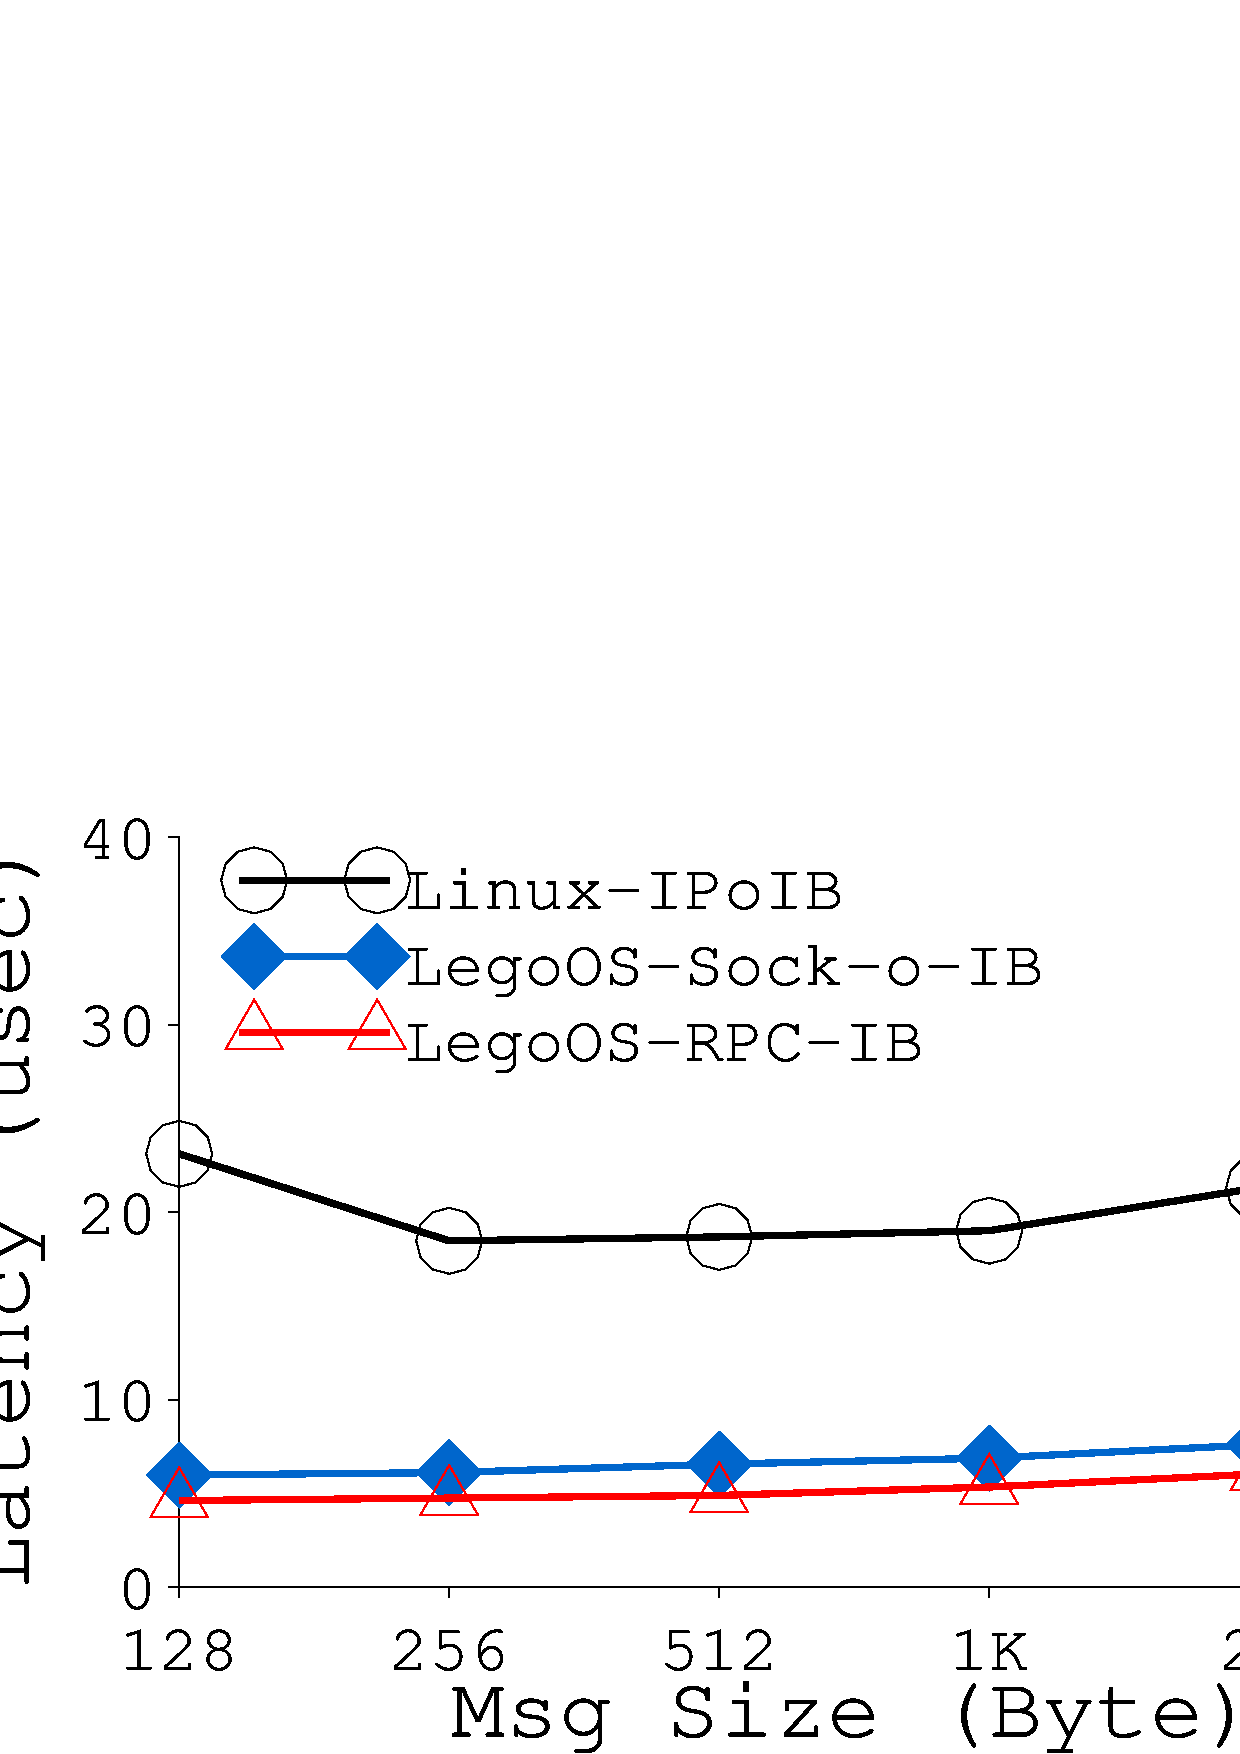
\includegraphics[width=1.0\columnwidth]{Figures/g_plot_LEGO_latency.pdf}}
\vspace{-0.1in}
\mycaption{fig-net-latency}{Network Latency.}
{
%Lego raw RPC over IB and socket over IB, compared with Linux.
}
\end{center}
\end{minipage}
\begin{minipage}{0.50\columnwidth}
\vspace{0.13in}
\begin{center}
\centerline{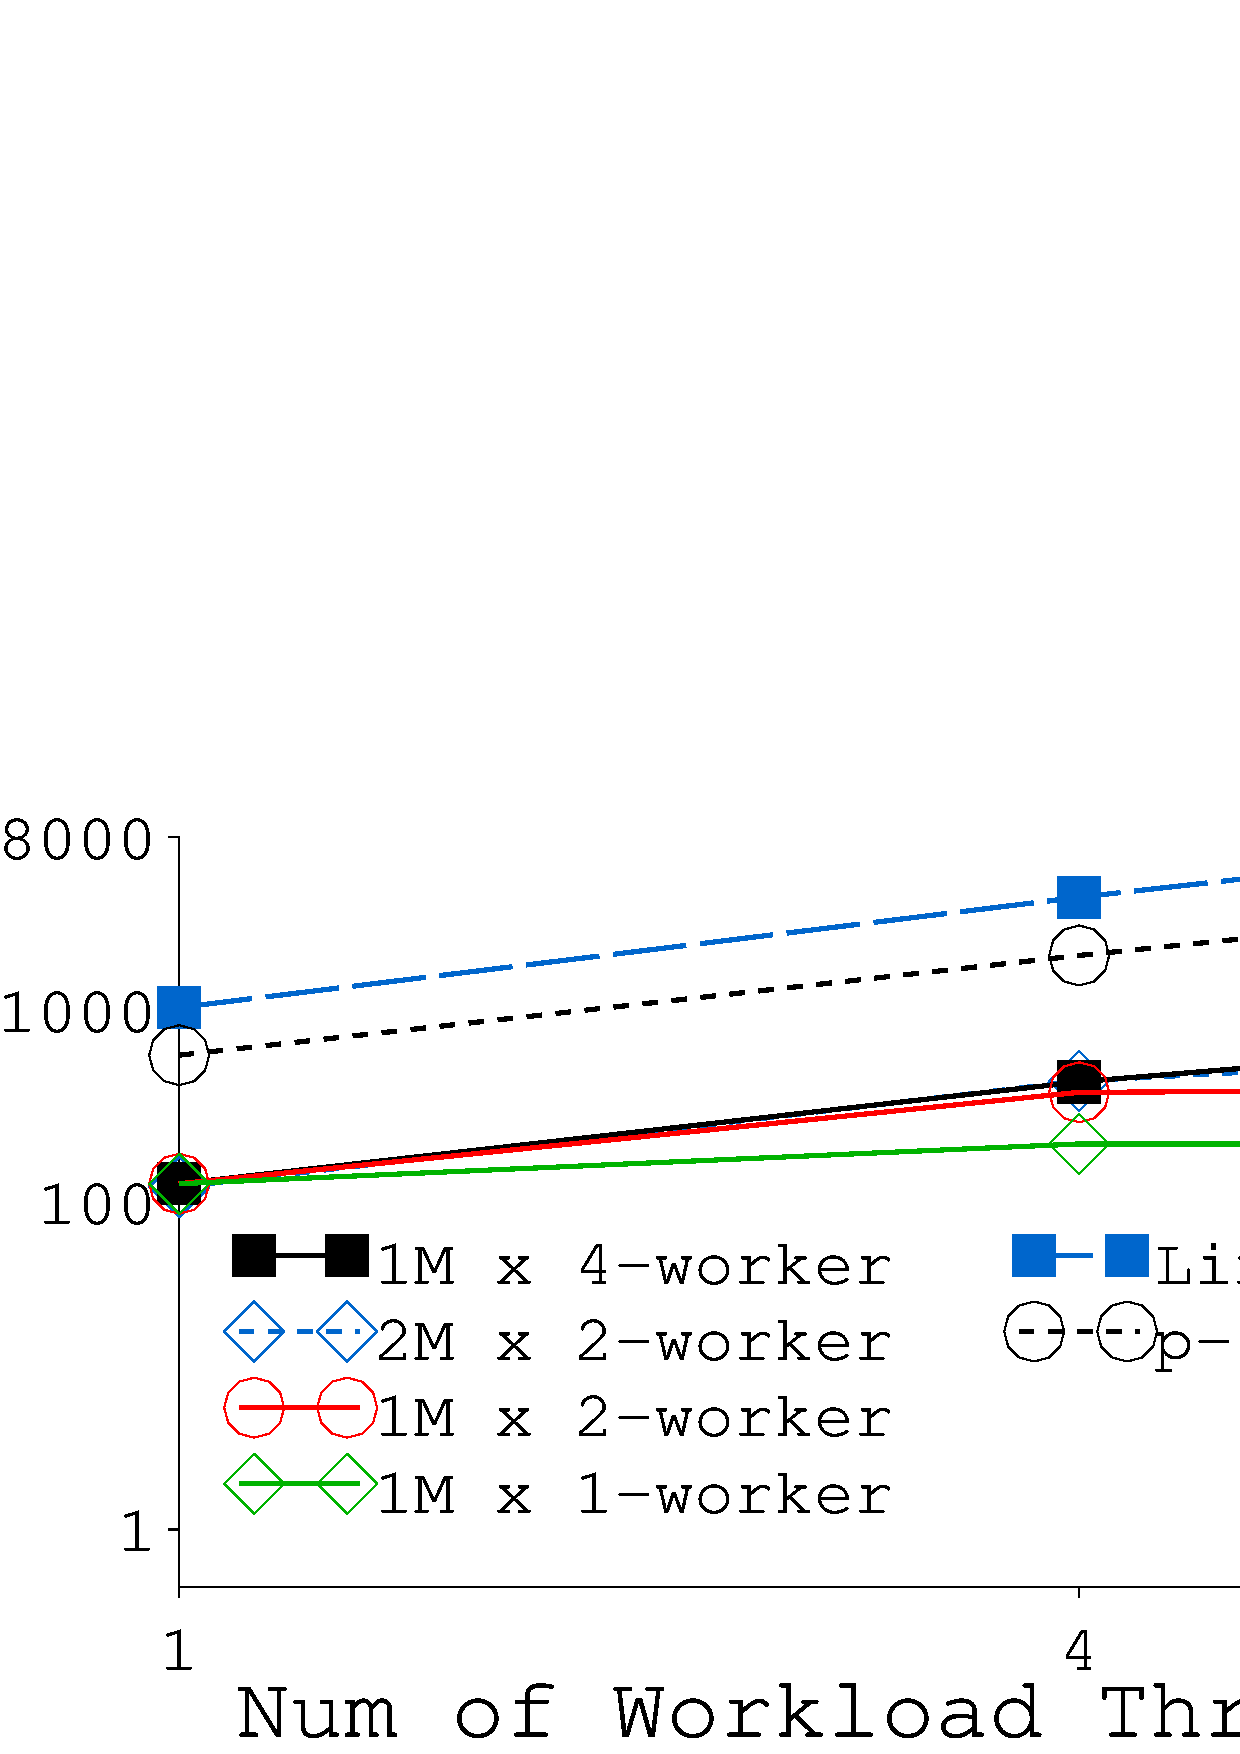
\includegraphics[width=1.0\columnwidth]{Figures/g_plot_LEGO_iops_memory.pdf}}
\vspace{-0.1in}
\mycaption{fig-iops-memory}{Memory Throughput.}
{
%Lego
}
\end{center}
\end{minipage}
\begin{minipage}{0.50\columnwidth}
\vspace{0.11in}
\begin{center}
\centerline{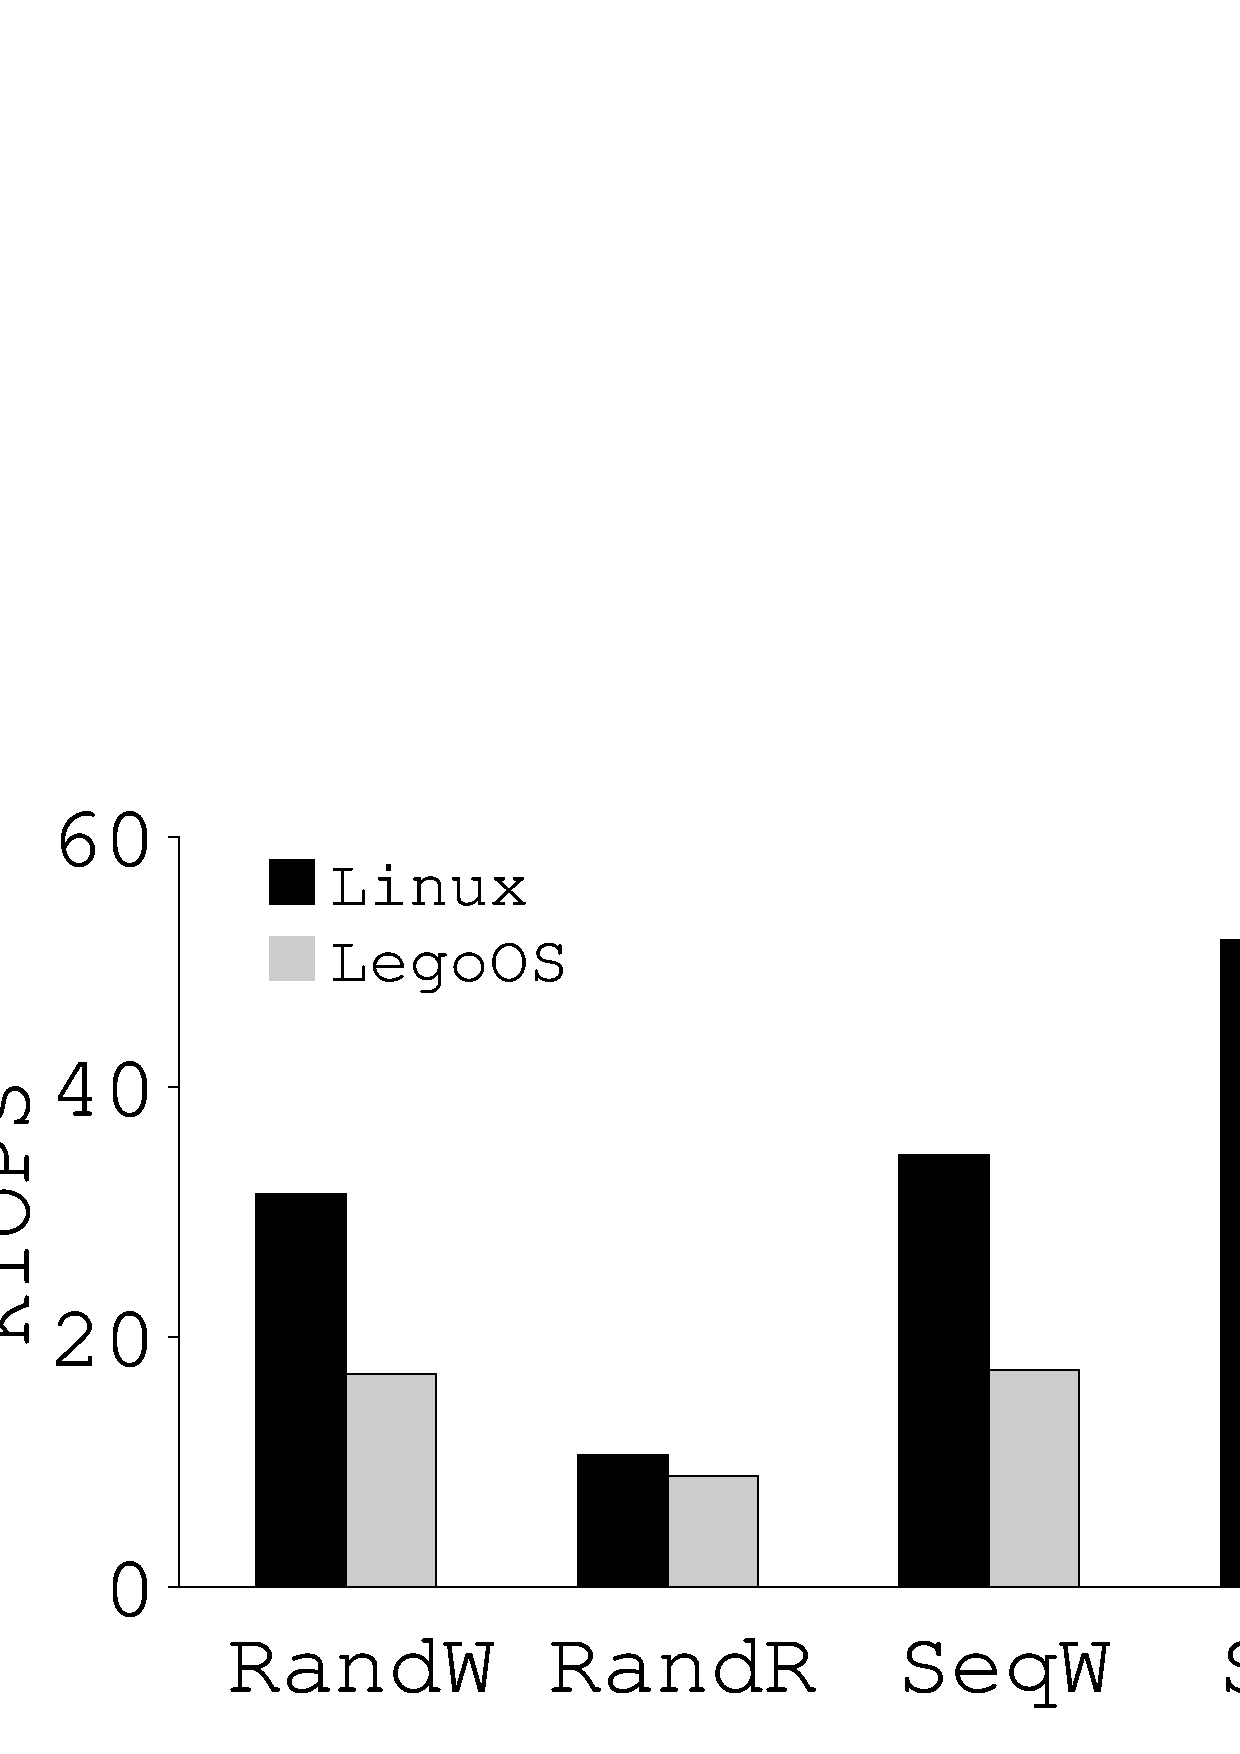
\includegraphics[width=1.0\columnwidth]{Figures/g_plot_LEGO_iops_storage.pdf}}
\vspace{-0.06in}
\mycaption{fig-iops-storage}{Storage Throughput.} 
{
%Random read/write performance.
}
\end{center}
\end{minipage}
\begin{minipage}{0.50\columnwidth}
\vspace{0.11in}
\begin{center}
\centerline{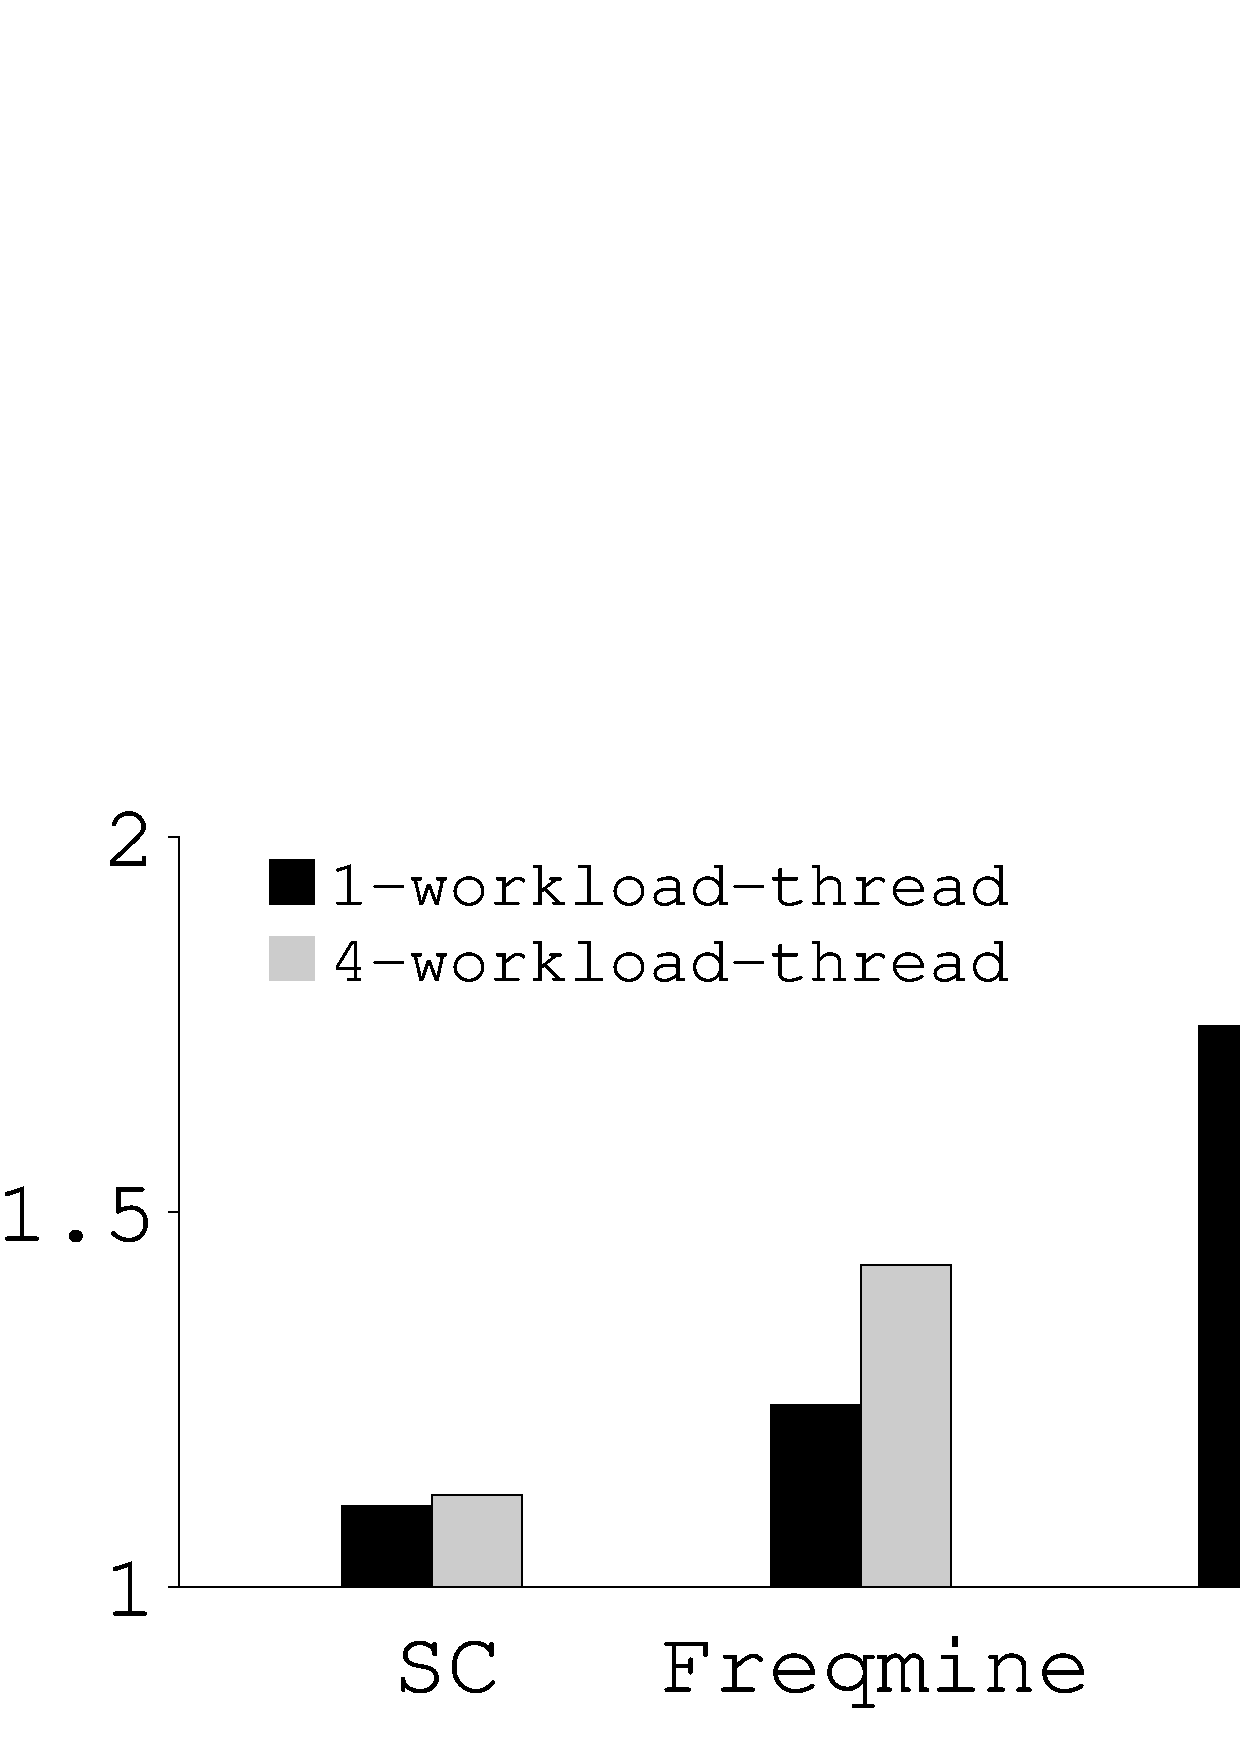
\includegraphics[width=1.0\columnwidth]{Figures/g_plot_LEGO_parsec.pdf}}
\vspace{-0.06in}
\mycaption{fig-parsec}{PARSEC Results.}
{
SC: StreamClsuter. BS: BlackScholes.
%TensorFlow and Phoenix running on Lego with different ExCache size configurations.
%Compared with running on Linux with limited memory.
}
\end{center}
\end{minipage}
\vspace{-0.1in}
\end{figure*}
}
